\section*{Funktionenr�ume und Bestapproximation Aufgaben mit L�sungen}\label{MA2-funktionenraeume-und-bestapproximation-loesungen}

\ifintegriereaufgaben Erkl�rungen und Beispiele, die zum Verst�ndnis der L�sungswege hilfreich sind, finden Sie im Skript\wennreferenzvorhanden{MA2-funktionenraeume-und-bestapproximation}{ (Abschnitt \abschnittsverweis{MA2-funktionenraeume-und-bestapproximation})} des Skripts.\fi

\begin{exercisebox}[Gram-Schmidtsches Orthogonalisierungsverfahren]
	Gegeben sind drei linear unabh�ngige Vektoren. Bestimmen Sie ein Orthonormalsystem.
	\[
		\boldsymbol v_1 = \left( \begin{array}{c} 1 \\ i \\ 0 \\ 0 \end{array}\right)\,,
		\boldsymbol v_2 = \left( \begin{array}{c} i \\ 0 \\ 0 \\ i \end{array}\right)\,,
		\boldsymbol v_3 = \left( \begin{array}{c} 1 \\ 0 \\ 1 \\ 0 \end{array}\right)\,.
	\]

\vspace{0.3cm}
\textbf{L�sung:} \newline

\vspace{0.2cm}
{Erinnerung:} Das Skalarprodukt und die Norm auf dem Vektorraum \(\mathbb C^n\) ist anders als das Skalarprodukt in \(\mathbb R^n\). Beispielsweise haben lautet das Skalarprodukt zwischen \(\boldsymbol v_1\) und \(\boldsymbol v_2\) bzw. die Norm von \(\boldsymbol v_1\):
\begin{eqnarray*}
	\langle \boldsymbol v_1, \boldsymbol v_2\rangle &=&  \boldsymbol v_1 \boldsymbol \cdot \overline{\boldsymbol v_2} = 1\cdot (- i)  + i\cdot 0 + 0\cdot 0 + 0\cdot (-i) = -i \\
	||\boldsymbol v_1|| = \sqrt{\boldsymbol v_1 \boldsymbol \cdot {\overline{\boldsymbol v}_1}} &=& \sqrt{1\cdot 1  + i\cdot (-i) + 0\cdot 0 + 0\cdot 0} = \sqrt{2}\,.
\end{eqnarray*}

\vspace{0.3cm}
Unsere Aufgabe besteht also darin basierend auf den drei gegebenen Vektoren drei Einheitsvektoren zu konstruieren, f�r die gilt \[ \langle \hat{\boldsymbol e}_i, \hat{\boldsymbol e}_j \rangle = \delta_{ij} = \begin{cases} 1, \quad &i=j \\  0, & i\not=j\end{cases} \]
Das Orthonormalsystem bestimmen wir in drei Schritten:
	\begin{enumerate}
		\item Wir bestimmen zu $\boldsymbol v_1$ einen Einheitsvektor $\hat {\boldsymbol e}_1$ mit  \( \hat {\boldsymbol e}_1 \parallel \boldsymbol v_1 \;\land\; ||\hat{\boldsymbol e}_1||= 1  \):
			\begin{eqnarray*}
				\Rightarrow \hat{\boldsymbol e}_1 = \frac{\boldsymbol v_1}{|| \boldsymbol v_1||} = \frac{1}{\sqrt{2}}\left( \begin{array}{c} 1 \\ i \\ 0 \\ 0\end{array}\right)
		\end{eqnarray*}
	\item Wir bestimmen zu $\boldsymbol v_2$ in zwei Schritten einen Einheitsvektor $ \hat {\boldsymbol e}_2$ mit  \( \hat {\boldsymbol e}_2 \perp \hat{\boldsymbol e}_1   \; \land \; \|\hat{\boldsymbol e}_2\| = 1 \):
			\begin{eqnarray*}
				 \boldsymbol e_2 &=& \boldsymbol v_2 - \langle \boldsymbol v_2, \hat{\boldsymbol e}_1\rangle \hat{\boldsymbol e}_1  = \left( \begin{array}{c} i \\ 0 \\ 0 \\ i \end{array}\right) - \frac{i}{2} \left( \begin{array}{c} 1 \\ i \\ 0 \\ 0\end{array}\right) = \frac12\left( \begin{array}{c} i \\ 1 \\ 0 \\ 2i\end{array}\right) \\
			\Rightarrow  \hat{\boldsymbol e}_2 &=& \frac{\boldsymbol e_2}{|| \boldsymbol e_2||} = \frac{1}{\sqrt{6}}\left( \begin{array}{c} i \\ 1 \\ 0 \\ 2i\end{array}\right)
		\end{eqnarray*}
	\item Wir bestimmen zu $\boldsymbol v_3$ einen Vektor $\boldsymbol e_3$ mit  \( \hat{\boldsymbol e}_3 \perp \hat{\boldsymbol e}_i, \; i=1,2 \; \land \; \|\hat{\boldsymbol e}_3\| = 1 \):
		\begin{eqnarray*}
			\boldsymbol e_3 &=& \boldsymbol v_3 - \langle \boldsymbol v_3, \hat{\boldsymbol e}_1\rangle \hat{\boldsymbol e}_1 - \langle \boldsymbol v_3, \hat{\boldsymbol e}_2\rangle \hat{\boldsymbol e}_2 = \left( \begin{array}{c} 1 \\ 0 \\ 1 \\ 0  \end{array}\right) - \frac{1}{2}\left( \begin{array}{c} 1 \\ i \\ 0 \\ 0\end{array}\right) - \frac{(-i)}{6}\left( \begin{array}{c} i \\ 1 \\ 0 \\ 2i\end{array}\right)
		= \frac13\left( \begin{array}{c} 1 \\ -i\\ 3 \\ -1 \end{array}\right)  \\
		\Rightarrow \hat{\boldsymbol e}_3 &=& \frac{\boldsymbol e_3}{|| \boldsymbol e_3||} = \frac{1}{\sqrt{11}}\left( \begin{array}{c} 1 \\ -i \\ 3 \\ -1\end{array}\right)
		\end{eqnarray*}
	\end{enumerate}
	Bemerkung: Das System aus den Vektoren \( \hat{\boldsymbol e}_1, \hat{\boldsymbol e}_2, \hat{\boldsymbol e}_3\) ist orthonormiert. Um eine Basis des \(\mathbb C^4\) zu erhalten, m�sste man das System noch um einen vierten Vektor erg�nzen, der zu den anderen orthogonal ist und L�nge eins hat.
\end{exercisebox}

\begin{exercisebox}[Basis] %https://www.lntwww.de/Aufgaben:Aufgabe_4.1:_Zum_Gram-Schmidt-Verfahren
	Bei der Digitalsignal�bertragung werden energiebegrenzte Signale betrachtet. Das Skalarprodukt zweier Signale bzw. die Norm eines Signals sind hierbei wie folgt definiert:
	\begin{eqnarray*}
		\langle s_i, s_k\rangle &=& \int\limits_{-\infty}^{\infty} s_i(t) \cdot s_k(t) \, \mathrm{d}t\,,\\[1ex]
		\|s\| &=& \sqrt{\langle s,s \rangle}\,.
	\end{eqnarray*}
	Betrachten Sie die folgenden drei energiebegrenzten Signale:
	\begin{center}
	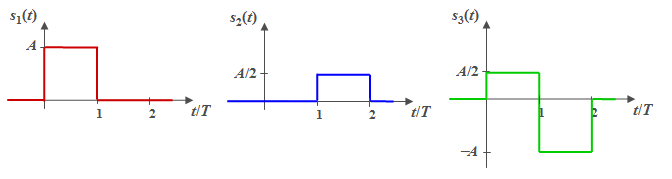
\includegraphics[width=0.7\textwidth]{../Mathematik_2/Bilder/funktionenraum_rechtecksignale_linearkombination.png}
\end{center}
	\begin{itemize}
		\item[(a)] Wie lauten die Abbildungsvorschriften der Signale $s_1, s_2$ und $s_3$?
		\item[(b)] Berechnen Sie die Normen der Signale $s_1$ und $s_2$.
		\item[(c)] Konstruieren Sie aus den Signalen $s_1$ und $s_2$ ein Orthonormalsystem.
		\item[(d)] Zerlegen Sie das Signal $s_3$ bez�glich des Orthonormalsystems und bestimmen Sie die vektoriellen Repr�sentanten der Ausgangssignale bez�glich des Orthonormalsystems.
	\end{itemize}
\vspace{0.3cm}
\textbf{L�sung:} \newline
\begin{itemize}
\item[(a)]
	\begin{eqnarray*}
		s_1: &t\mapsto& \begin{cases} 0, \quad &t\leq 0\,,\\
			A, \quad &0<t\leq 1\,,\\
			0,\quad &t>1\,,
		\end{cases}\\
		s_2: &t\mapsto& \begin{cases} 0, \quad &t\leq 1\,,\\
			A/2, \quad &1<t\leq 2\,,\\
			0,\quad &t>2\,,
		\end{cases}\\
		s_3: &t\mapsto& \begin{cases} 0, \quad &t\leq 0\,,\\
			A/2, \quad &0<t\leq 1\,,\\
			-A, \quad &1<t\leq 2\,,\\
			0,\quad &t>2\,.
		\end{cases}
	\end{eqnarray*}
\item[(b)] Wir berechnen die L�nge der Signale mit dem angegebenen Skalarprodukt:
	\begin{eqnarray*}
		|s_1|^2 &=&  \langle s_1, s_1 \rangle = \int\limits_{-\infty}^\infty s_1(t)\cdot s_1(t) \, \mathrm{d} t = \int\limits_0^1 A^2 \mathrm{d}t = A^2 \;  \Rightarrow |s_1| = |A|\,,\\
		|s_2|^2 &=&  \langle s_2, s_2 \rangle = \int\limits_{-\infty}^\infty s_2(t)\cdot s_2(t) \, \mathrm{d} t = \int\limits_1^2 \left( \dfrac{A}{2} \right)^2\, \mathrm{d}t = \dfrac{A^2}{4} \;  \Rightarrow |s_2| = \left| \dfrac{A}{2}\right|\,.
	\end{eqnarray*}
	Bemerkung: hieran sehen, wir dass die Signale \(s_1\) und \(s_2\) nicht normiert sind.

\item[(c)] Wir �berpr�fen, ob die Signale bez�glich des gegebenen Skalarprodukts orthogonal zueinander sind, indem wir das Skalarprodukt berechnen:
	\[ \langle s_1, s_2 \rangle = \int\limits_{-\infty}^\infty s_1(t) \cdot s_2(t) \,\mathrm d t =  0\,, \]
	Die Intervalle, auf denen die Signale von Null verschieden sind, �berplappen sich nicht und damit ist das Integral null. Die Signale sind orthogonal. Um eine Orthonormalbasis aus \(s_1\) und \(s_2\) zu konstruieren, m�ssen die Signale nur noch normiert werden:

	\[
		\begin{cases}
			\hat s_1(t) = \displaystyle{\frac{ s_1(t)}{|s_1|}} = \displaystyle{\frac{ s_1(t)}{A}}\,,\\
			\hat s_2(t) = \displaystyle{\frac{ s_2(t)}{|s_2|}} = \displaystyle{\frac{ s_2(t)}{A/2}}\,.
	\end{cases} \]
\item[(d)] Das Signal \(s_3\) kann in eine lineare Kombination aus \(\hat s_1\) und \(\hat s_2\) zerlegt werden  \[ s_3(t) = \lambda_1 \cdot \hat s_1(t) + \lambda_2 \cdot \hat s_2(t)\] mit
	\begin{eqnarray*}
		\lambda_1 &=& \langle s_3, \hat s_1\rangle = A/2\\
		\lambda_2 &=& \langle s_3, \hat s_2\rangle = -A
	\end{eqnarray*}

	Die vektoriellen Repr�sentanten der Signale in dem zweidimensionalen Vektorraum, der von den Funktionen $\hat s_1$ und $\hat s_2$ aufgespannt wird, lauten
	\[\boldsymbol s_1 = \left(\begin{array}{c} A\\ 0\end{array}\right), \;
	\boldsymbol s_2 = \left(\begin{array}{c} 0\\ A/2\end{array}\right), \;
\boldsymbol s_3 = \left(\begin{array}{c} A/2\\ -A/2\end{array}\right)\,. \]
	\begin{center}
	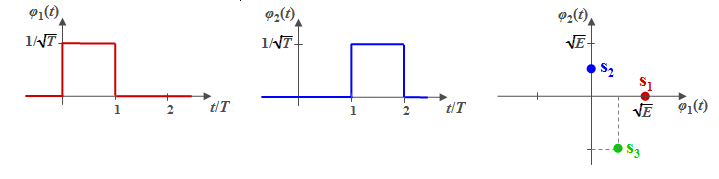
\includegraphics[width=0.7\textwidth]{../Mathematik_2/Bilder/funktionenraum_rechtecksignale_orthonormale_basis.png}
\end{center}
\end{itemize}
\end{exercisebox}


\begin{exercisebox}[Bestapproximation] %A.Z. Anwendungen
	Gegeben seien die Funktionen $f_1, f_2, f_3 \in \mathcal C([-\pi,\pi], \mathbb R)$ mit
	\[ f_1: x\mapsto 1, \quad f_2: x\mapsto \cos(x), \quad f_3: x\mapsto \sin(x)\]
	\begin{itemize}
		\item[(a)] Zeigen Sie, dass die Funktionen paarweise orthogonal sind bez�glich des Skalarprodukts
			\[ \langle f, g\rangle : = \int_{-\pi}^{\pi} f(x) \cdot g(x) \, \mathrm{d}x \]
		\item[(b)] Berechnen Sie die Bestapproximation $\tilde f \in \mathcal C([-\pi,\pi],\mathbb R)$ von $f:x\mapsto x^2$ bez�glich $f_i$, $i=1,2,3$ und zeichnen Sie $f$ und $\tilde f$.
		\item[(c)] Zeigen Sie, dass die folgenden Funktionen orthogonal sind\[ \cos(k\cdot x), \, k\in \mathbb N_0, \quad \sin(k\cdot x),  \, k\in \mathbb N\,.\]
	\end{itemize}

\vspace{0.3cm}
\textbf{L�sung:} \newline
\begin{itemize}
	\item[(a)] Die Funktionen sind zueinander orthogonal, denn
		\begin{eqnarray*}
			\langle f_1, f_2\rangle = \int_{-\pi}^\pi \cos(x)\,\mathrm{d}x = \big[ \sin(x) \big]_{-\pi}^\pi  = 0\,,\\
			\langle f_1, f_3\rangle = \int_{-\pi}^\pi \sin(x)\,\mathrm{d}x = \big[ -\cos(x) \big]_{-\pi}^\pi  = 0\,,\\
			\langle f_2, f_3\rangle = \int_{-\pi}^\pi \cos(x)\cdot \sin(x)\,\mathrm{d}x = \big[ \frac12 \sin^2(x) \big]_{-\pi}^\pi  = 0\,.
		\end{eqnarray*}
		Leicht k�nnen wir sie auch normieren:
		\begin{eqnarray*}
			||f_1||^2 &=& 2\pi \Rightarrow \hat f_1: x\mapsto \frac{1}{\sqrt{2\pi}} \\
			||f_2||^2 &=& \pi \Rightarrow \hat f_2: x\mapsto \frac{1}{\sqrt{\pi}} \cos(x)\,,\\
			||f_3||^2 &=& \pi \Rightarrow \hat f_3: x\mapsto \frac{1}{\sqrt{\pi}} \sin(x)\,.
		\end{eqnarray*}
	\item[(b)] Die Bestapproximation von \(f\) bez�glich des Unterraums, der von den Funktionen \( \{ \hat f_1, \hat f_2, \hat f_3\}\) aufgespannt wird lautet:
		\begin{eqnarray*} \tilde f(x) &=& \langle f, \hat f_1\rangle \hat f_1 + \langle f, \hat f_2\rangle \hat f_2  + \langle f, \hat f_3\rangle \hat f_3 \\
		&=& \frac{1}{2\pi} \int\limits_{-\pi}^\pi x^2\,\mathrm{d}x + \frac{1}{\pi} \left(\int\limits_{-\pi}^\pi x^2\cdot \cos(x)\,\mathrm{d}x\right) \cos(x)  + \frac{1}{\pi}\left( \int\limits_{-\pi}^\pi x^2\cdot \sin(x)\,\mathrm{d}x \right) \sin(x)\\
	&=& \frac{\pi^2}{3} - 4\cos(x)\,.\end{eqnarray*}
		Denken Sie daran, dass sich Integrale deren Integrand ein Produkt aus Polynom und trigonometrischer Funktion ist mit mehrfacher partieller Integration l�sen l��t.
	\begin{center}
	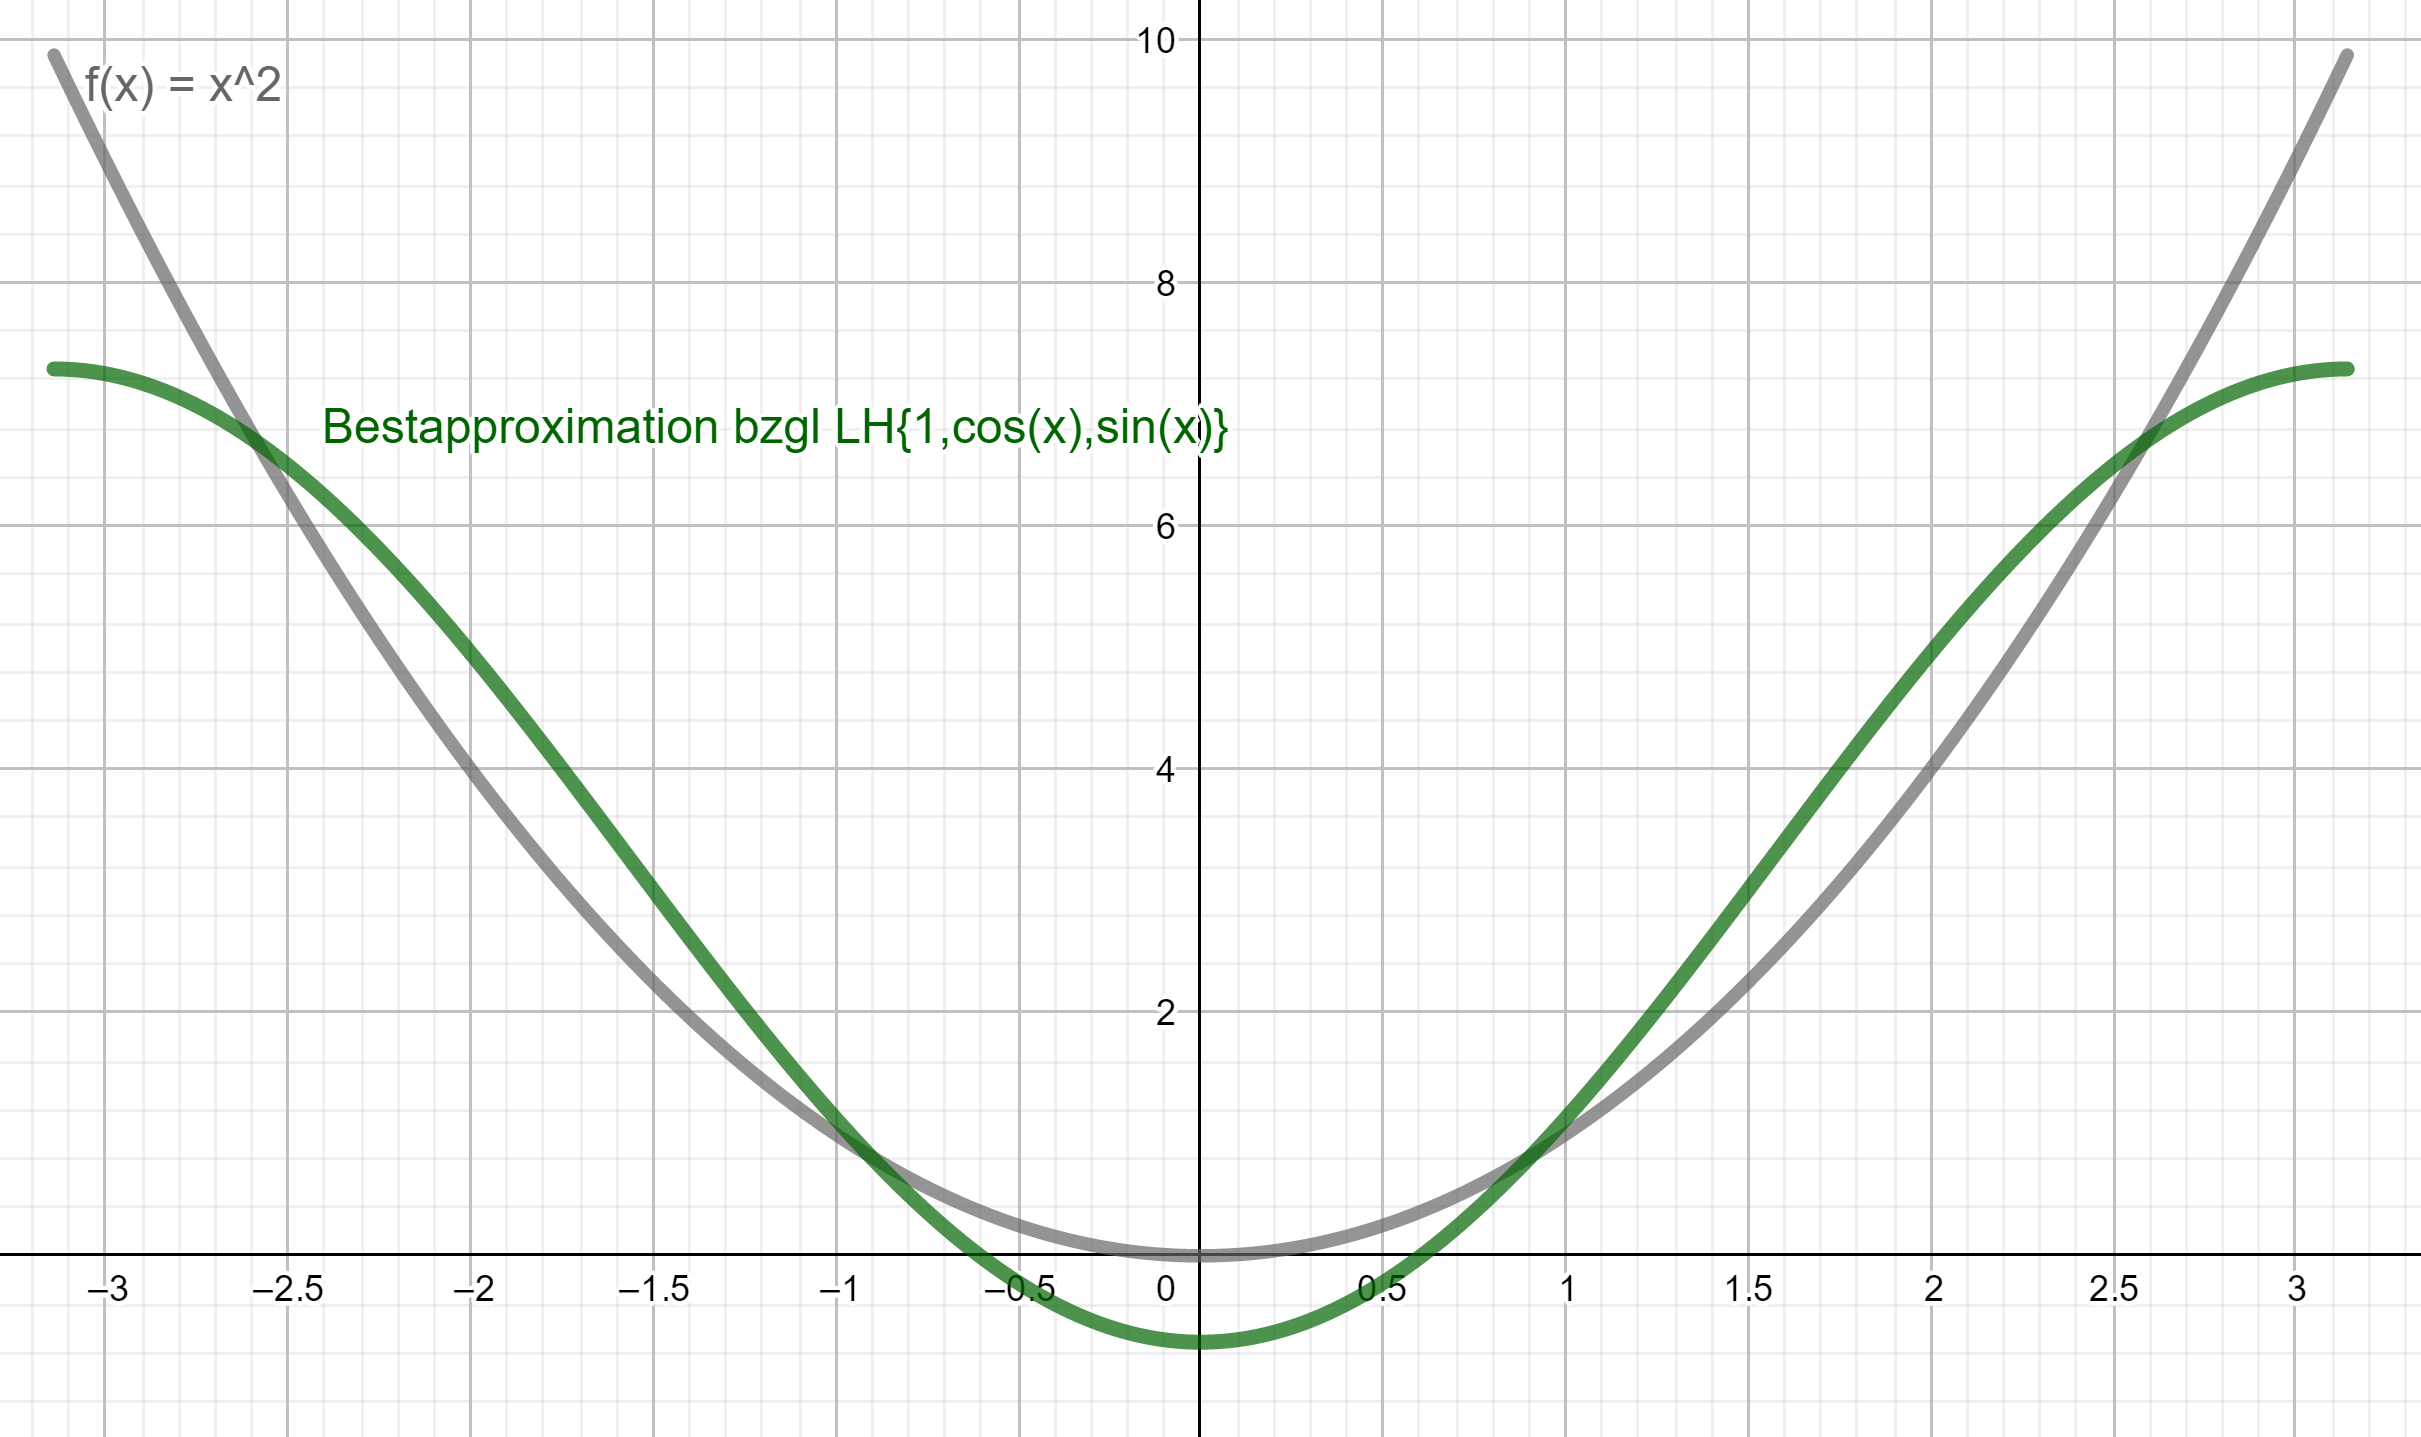
\includegraphics[width=0.8\textwidth]{../Mathematik_2/Bilder/bestapproximation_quadratfunktion_durch_cosinus.png}
\end{center}
	\item[(c)]  Man verwendet die Formeln
		\begin{eqnarray*}
			\cos(\alpha)\cdot \cos(\beta) &=& \frac12 \left( \cos( \alpha - \beta) + \cos(\alpha + \beta)\right) \\
			\sin(\alpha)\cdot \sin(\beta) &=& \frac12 \left( \cos( \alpha - \beta) - \cos(\alpha + \beta)\right) \\
			\sin(\alpha)\cdot \cos(\beta) &=& \frac12 \left( \sin( \alpha - \beta) + \sin(\alpha + \beta)\right)
		\end{eqnarray*}
	\end{itemize}
\end{exercisebox}



